\documentclass[border=6pt]{standalone}
\usepackage{tikz}

\definecolor{mut}{HTML}{0072B2}

\begin{document}
\pagecolor{white}
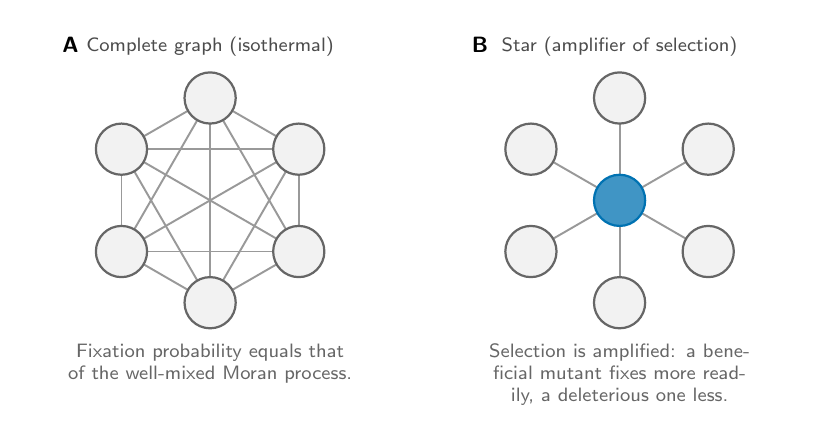
\begin{tikzpicture}[
    font=\sffamily,
    vert/.style={circle, draw=black!60, line width=0.8pt, fill=black!5,
                 minimum size=6.5mm, inner sep=0pt},
    edge/.style={black!40, line width=0.7pt},
    lab/.style={font=\sffamily\scriptsize, text=black!60, align=center},
    panel/.style={font=\sffamily\footnotesize\bfseries, anchor=north west},
    subcap/.style={font=\sffamily\scriptsize, text=black!70, align=center},
]

% ---- Panel A: complete graph (isothermal) ----
\begin{scope}[shift={(0,0)}]
    \node[panel] at (-2.0,2.2) {A};
    \node[subcap] at (0,1.95) {Complete graph (isothermal)};
    \foreach \i in {0,...,5} { \coordinate (A\i) at ({90+60*\i}:1.3); }
    \foreach \i in {0,...,5} {
        \foreach \j in {0,...,5} { \ifnum\i<\j \draw[edge] (A\i)--(A\j); \fi }
    }
    \foreach \i in {0,...,5} { \node[vert] at (A\i) {}; }
    \node[lab, anchor=north, text width=4.4cm] at (0,-1.7)
        {Fixation probability equals that of the well-mixed Moran process.};
\end{scope}

% ---- Panel B: star graph (amplifier) ----
\begin{scope}[shift={(5.2,0)}]
    \node[panel] at (-2.0,2.2) {B};
    \node[subcap] at (0,1.95) {Star (amplifier of selection)};
    \coordinate (centre) at (0,0);
    \foreach \i in {0,...,5} { \coordinate (S\i) at ({90+60*\i}:1.3); }
    \foreach \i in {0,...,5} { \draw[edge] (centre)--(S\i); }
    \foreach \i in {0,...,5} { \node[vert] at (S\i) {}; }
    \node[vert, fill=mut!75, draw=mut, text=white] at (centre) {};
    \node[lab, anchor=north, text width=4.4cm] at (0,-1.7)
        {Selection is amplified: a beneficial mutant fixes more readily,
         a deleterious one less.};
\end{scope}
\end{tikzpicture}
\end{document}
